%% ==============================
\chapter{Single-bidder and Single-item Deterministic Auctions}
\label{ch:DAPX}
%% ==============================
In this chapter, we evaluate DAPX under single-bidder and single-item deterministic auction experiment with some well-known probability distribution. We use Myerson optimal acution as our auction mechanism, that seller make a reserve price for the item and if the bidder's bid higher than the reserve price, she gets the item and charged by the reserve price, otherwise the item remains un-sale. This is also called \textit{take-it-or-leave-it} auction. We start with some Definitions and euqtions from Robust paper.
\begin{definition}[Function $\rho$]
	\label{definition:functionD}
	For any $r \geqslant 0$, let $\rho(r) = \rho_D$ be the unique positive solution of equation
	\begin{equation}\notag
	\frac{(\rho - 1)^3}{(2\rho - 1)^2} = r^2
	\end{equation}
\end{definition}
where $r = \frac{\sigma}{u}$ is called \textit{coefficient of variation (CV)}. If we look at the left-hand side expression $\frac {(\rho_{D}-1)^{3}}{(2\rho_{D}-1)^{2}}$ is increasing and goes from 0 at $\rho_{D} = 1$, and to $\infty$ at $\rho_{D} \rightarrow \infty$, so that for any non-negative $r$ there is a unique solution $\rho_{D} \in [1,\infty)$ to the above equation. \\
The paper proposed a reserve price in terms of $\rho_D$ for the \textit{take-it-or-leave-it} auction 
\begin{equation}
\label{equation:rhoD}
	p_D =  \mu \cdot \frac{\rho_{D}}{2\rho_{D}-1} 
\end{equation}
where $\rho_{D}$ is given in Definition \ref{definition:functionD}.\\We know from Myerson [50] that for single-item settings the optimum revenue can be achieved by a deterministic mechanism by setting a reserve price $p$ and we can write the optimal revenue
\begin{equation}
\text{OPT}(F) = \sup_{p \geqslant 0} \text{REV}(p;F) = \sup_{p \geqslant 0} p \times \left(1-F(p-)\right) 
\end{equation}
where $F(p-) = Pr[x<p]$. \\
We denote $\text{OPT}(F)$ as Myerson optimal operator. We can use $\text{OPT}(F)$ to determine the optimal reserve price. Given a valuation probability distribution $F$, we are able to find a reserve price $p =\displaystyle\ \arg \max_{\substack{p \geqslant 0}} \ p \times \left(1-F(p-)\right)$, and we denote this price as optimal reserve price $p_{opt}$. Our experiment simulates over 100000 \textit{take-it-or-leave-it} auctions with reserve price $p_D$ and $p_{opt}$ separately, and we compute the expected revenues. We denote the expected revenue with reserve price $p_D$ as $\text{REV}(F)$, and the expected revenue with reserve price $p_{opt}$ as $\text{OPT}(F)$. Thus our experimental DAPX for distribution $F$ is:
DAPX = $\frac{\text{OPT}(F)}{\text{REV}(F)}$.\\
Procedure \ref{alg:auctionexperiment} shows our design for the auction experiment. Detailed Python code can be viewed on Github*.
\begin{algorithm}
%\floatname{algorithm}{Auction Experiment Procedure}
\caption{\textbf{Auction Experiment}} \label{alg:auctionexperiment}
\begin{algorithmic}[1]
	\Procedure{Auction Experiment}{$p,n,F$} \Comment{n = number of experiments}
	
		\State bid\_data $\gets$ $n$ random numbers generated from distribution $F$ 
		\State $\text{REV}(F) = 0$
		\For{each $bid$ in bid\_data}\Comment{stop until the last bid in bid\_data}                    
			\If{$bid \geqslant p$}
				\State $\text{REV}(F)$ = $\text{REV}(F)$ + $p$ \Comment{bidder wins and pay price $p$}
			\EndIf
			
		\EndFor
		\State \Return $\frac{\text{REV}(F)}{n}$
	\EndProcedure	
\end{algorithmic}

\end{algorithm}

\section{Uniform distribution}
For an uniform distribution $U[a,b], 0\leqslant a\leqslant b$, we know:
\begin{itemize}
	\item mean $\mu = \frac{b+a}{2}$ and $\sigma^{2} = \frac{(b-a)^{2}}{12}$
	\item CDF $F(x) = \frac {x-a}{b-a} $ 
	\item PDE $f(x) = \frac{1}{b-a}$
\end{itemize}
Using Myerson optimal operator, we can write:
\begin{equation}\notag
\text{OPT}(F) = \sup_{p \geqslant 0} \text{REV}(p;F) = \sup_{p \geqslant 0} p \times (1-\frac {p-a}{b-a}) 
\end{equation}
$p \times (1-\frac {p-a}{b-a})$ is a concave function, therefore, there exists a maximum point. Then we take its first derivative 
\begin{equation}\notag
	(p \times (1-\frac {p-a}{b-a}))^{'}  = (\frac {pb-p^2}{b-a})^{'} = \frac {b-2p}{b-a} 
\end{equation}
Because $p \in [a, b]$, we need to divide it into two cases.
\begin{itemize}
	\item Case 1: if $\frac{b}{2} < a, \frac {b-2p}{b-a}$ is negative then it means this function is monotone decreasing on $[a, b]$. Thus when $p = a$, we get OPT($F$). 
	\item Case 2: if $\frac{b}{2} \geqslant a $, then the maximum expected revenue can be achieved when $p = \frac{b}{2}$ 
\end{itemize}
Combine two cases above, when $p_{opt} =\text{max} \{a, \frac{b}{2} \}$, we have $\text{OPT}(F) =p_{opt} \times (1-\frac {p_{opt}-a}{b-a})$.\\
For a given uniform distribution, i.e. $a$ and $b$ are known, therefore $r^{2}$ is also known: $r^{2} = (\frac{\sigma}{u})^{2} = \frac{(b-a)^{2}}{3(b+a)^{2}}$, then we can determine $\rho_{D}$ by solving equation in Definition \ref{definition:functionD} and compute reserve price $p_D$ using Equation \ref{equation:rhoD}, Then our expected revenue
\begin{equation}\notag
	\text{REV} (F) = \frac{\rho_{D}}{2\rho_{D}-1}\cdot \mu \cdot (1-\frac{\frac{\rho_{D}}{2\rho_{D}-1}\cdot \mu -a}{b-a})
\end{equation}
However, we do not determine $\text{OPT}(F)$ and $\text{REV}(F)$ using above expressions during the experiments. We only use their reserve price $p_{opt}$ and $p_D$ during the experiments.

\subsection{The Bound of $r$ and DAPX}
Based on our experiments, we notice that no matter how we change $a$ and $b$, the \textit{coefficience of variation} $r$ of uniform distribution is way smaller than 1. Which is expected, as uniform distribution is well defined distribution and actually indeed we can write r in terms of $a$ and $b$ explicitly:
\begin{equation}\notag
r = \frac{\mu}{\sigma} = \frac {b-a}{\sqrt{3}(a+b)} = \frac {a+b-2a}{\sqrt{3}(a+b)} = \frac {1}{\sqrt{3}} (1-  \frac {2}{1+\frac{b}{a}})
\end{equation} 
when a = 0. then $r = \frac {1}{\sqrt{3}}$, otherwise, when $b \rightarrow \infty$ and $a\leqslant b$, we can have:

\begin{equation}\notag
\sup r = \displaystyle{\lim_{\frac{b}{a} \to \infty}}(\frac {1}{\sqrt{3}} (1-  \frac {2}{1+\frac{b}{a}})) = \frac {1}{\sqrt{3}}  
\end{equation} 
as we can see the CV of uniform distribution is at most $\frac {1}{\sqrt{3}}$.

From  equation \ref{equation:rhoD}, $\rho_D$ is monotonically increasing with $r$, then $\rho_D$ is also upper bounded. we can compute its upper bound using numerical solver by setting $r = \frac {1}{\sqrt{3}}$ in equation \ref{equation:rhoD}. We know the equation of computing the reserve price, $p_D =  (\frac{a+b}{2}) \cdot \frac{\rho_{D}}{2\rho_{D}-1} =\frac{1}{2-\frac{1}{\rho_D}}\cdot (\frac{a+b}{2})$. \\
Now let's write DAPX explicitly, when $\frac{b}{2} \geqslant a$ so $p_{opt} = \frac{b}{2}$ : 
\begin{equation}\notag
\text{DAPX} = \frac{\text{OPT}(F)}{\text{REV}(F)} =  \frac{\frac{b^{2}}{4(b-a)}}{\frac{\rho_{D}}{2\rho_{D}-1}\cdot \mu \cdot (1-\frac{\frac{\rho_{D}}{2\rho_{D}-1}\cdot \mu -a}{b-a})}
\end{equation} 

simplified we get 
\begin{equation}\notag
\text{DAPX}=\frac{b^{2}}{\frac{2\rho_{D}}{2\rho_{D}-1}\cdot 2\mu \cdot(b-\frac{\rho_{D}}{2\rho_{D}-1}\cdot \mu)}
\end{equation} 

subsititute $b = \sqrt{3}\sigma + \mu $
\begin{equation}\notag
	\begin{split}	
		\text{DAPX} &=\frac{( \sqrt{3}\sigma + \mu)^{2}}{\frac{2\rho_{D}}{2\rho_{D}-1}\cdot 2\mu \cdot( \sqrt{3}\sigma + \mu-\frac{\rho_{D}}{2\rho_{D}-1}\cdot \mu)} \\&= \frac{\mu^2 \cdot( \sqrt{3}r +1)^{2}}{\frac{2\rho_{D}}{2\rho_{D}-1}\cdot 2\mu^2 \cdot( \sqrt{3}r+ 1-\frac{\rho_{D}}{2\rho_{D}-1})}\\ 
		&= \frac{ ( \sqrt{3}r +1)^{2}}{4 \cdot \frac{ \rho_{D}}{2\rho_{D}-1}\cdot( \sqrt{3}r+ 1-\frac{\rho_{D}}{2\rho_{D}-1})}	
	\end{split}
\end{equation} 

when  $\frac{b}{2} \leqslant a$ so $p_{opt} = a$ 
\begin{equation}\notag
\text{DAPX} = \frac{\text{OPT}}{\text{REV}} =  \frac{a}{\frac{\rho_{D}}{2\rho_{D}-1}\cdot \mu \cdot (1-\frac{\frac{\rho_{D}}{2\rho_{D}-1}\cdot \mu -a}{b-a})}
\end{equation} 

simplified we get 
\begin{equation}\notag
\text{DAPX}=\frac{a(b-a)}{\frac{\rho_{D}}{2\rho_{D}-1}\cdot \mu \cdot(b-\frac{\rho_{D}}{2\rho_{D}-1}\cdot \mu)}
\end{equation} 
subsititute $b =  \mu +\sqrt{3}\sigma $ and $a  = \mu - \sqrt{3}\sigma$
\begin{equation}\notag
\begin{split}	
	\text{DAPX} &=\frac{2\sqrt{3}\sigma (\mu - \sqrt{3}\sigma)}{\frac{\rho_{D}}{2\rho_{D}-1}\cdot \mu \cdot( \sqrt{3}\sigma + \mu-\frac{\rho_{D}}{2\rho_{D}-1}\cdot \mu)} \\&= \frac{\mu^2 \cdot r( 1-\sqrt{3}r )}{\mu^2 \cdot \frac{\rho_{D}}{2\rho_{D}-1}\cdot( \sqrt{3}r+ 1-\frac{\rho_{D}}{2\rho_{D}-1})}\\ &= \frac{r( 1-\sqrt{3}r )}{\frac{\rho_{D}}{2\rho_{D}-1}\cdot( \sqrt{3}r+ 1-\frac{\rho_{D}}{2\rho_{D}-1})}
\end{split}
\end{equation} 

Below we represent the result in \cref{fig:uniform_dapx}, which compares DAPX of uniform distribution against theoretical value $\rho_D$ from the paper with different $r$ values.(show example, set a =1, change r value, since for each r there is a corresponding value of b, which is a valid uniform distribution, then we can get following plot


$ \frac{ \rho_{D}}{2\rho_{D}-1} = \frac{1}{2-\frac{1}{\rho_D}}$ as $\rho_D \geqslant 1$ because optimal revenue is always greater than the expected revenue, then $\frac{ \rho_{D}}{2\rho_{D}-1} \leqslant 1$. 
$\rho_d$ is also a function of $r$, it seems that DAPX is a quadratic equation in terms of $r$????? not too sure, since I cannot derive the pd using r
\textbf{note}: another interesting things when a uniform ditribution has $\frac{b}{a} = 2.44224957$, then DAPX = 1, by setting $p = p_{opt} $ which is equavlent to $\frac{\rho_{D}}{2\rho_{D}-1}\cdot (\frac{a+b}{2}) = \frac{b}{2}$ then solving equation \ref{equation:rhoD}.
\begin{figure}[H]
	\centering
	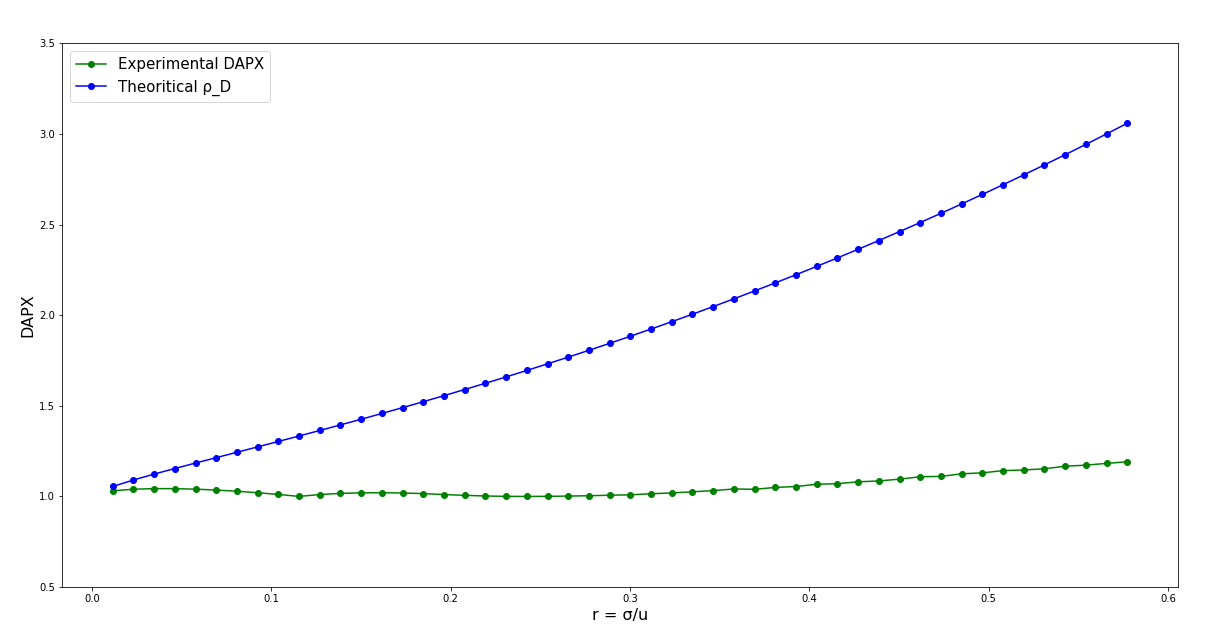
\includegraphics[width=1\textwidth]{uniform_dapx}
	\caption{DAPX of uniform distribution versus $\rho_{D}$}
	\label{fig:uniform_dapx}
\end{figure}



\section{Exponential and Poisson distribution}

These two distributions have very special property that the mean and the standard deviation are the same, which results in constant CV, for exponential distribution $r = \frac{\sigma}{\mu} = \frac{\frac{1}{\lambda}}{\frac{1}{\lambda}} = 1$ and for poisson distribution $r = \frac{\sigma}{\mu} = \frac{\lambda}{\lambda} = 1$, therefore $\rho_D$ is also constant by solving equation \ref{equation:rhoD}. Thus from these two distributions we cannot find a useful relation between DAPX and $r$. 

We can still perform some insight of this type distribution, and let us look at exponential distribution for example. For any exponential distribution, we denote as $exp(\lambda)$, its mean and standard deviation are $\frac{1}{\lambda}$, then using Meyerson optimal operator, we can determine the optimal reserve price is $\frac{1}{\lambda}$ and the optimal revenue is $\frac{1}{\lambda e}$. Let's denote $\hat{\rho_D}$ as the the value of $\rho_D$ when $r = 1$, and our expected revenue is $\frac{\hat{\rho_D}}{\lambda (2\hat{\rho_D} - 1)}e^{- \frac{\hat{\rho_D}}{(2\hat{\rho_D} - 1)}}$, then:

\begin{equation}\notag
\begin{split}	
	\text{DAPX} &= \frac{\text{OPT}(F)}{\text{REV}(F)} \\&= \frac{\frac{1}{\lambda \cdot e}}{\frac{\hat{\rho_D}}{\lambda (2\hat{\rho_D} - 1)}e^{- \frac{\hat{\rho_D}}{(2\hat{\rho_D} - 1)}}} \\&= \frac{1}{\frac{\hat{\rho_D}}{(2\hat{\rho_D} - 1)}e^{1- \frac{\hat{\rho_D}}{(2\hat{\rho_D} - 1)}}}
\end{split}
\end{equation} 
From above expression we can see DAPX is indepedent of $\lambda$, and it is a constant as well. 
we will not explore any futher on these two distributions.


\section{Truncated Normal distribution} \label{Normal distribution} 
Another interesting probability distribution to explore is the truncated normal distribution. The definition of truncated normal distribution is: suppose X is from a normal distribution with mean $\hat{\mu}$ and variance $\hat{\sigma}^2$ and lies within the interval [$a,b$], then X conditional on $a \leqslant X  \leqslant b$ has a truncated normal distribution TN($\hat{\mu}, \hat{\sigma^2}, a,b$). Here we assume $\hat{\mu} \geqslant0 $, because if $\hat{\mu} <0$, that means the density function of truncated normal distribution is monotone decreasing, which means we have high probability of low valuation bidders and low probability of high valuation bidders. This kind of characteristics can be captured by another probability distribution which we introduce in the next section called Pareto distribution. To notice here $\hat{\mu}$ and $\hat{\sigma}$ are the mean and standard deviation of the normal distribution before the truncation, and we denote $\mu$ and $\sigma$ are the mean and standard deviation of the truncated normal distribution. We also assume the truncated range is [0, $\infty$), thus set $a = 0$ and $b = \infty$. The corresponding PDF and CDF of TN($\hat{\mu}, \hat{\sigma}^2, 0,\infty$): (using the notation from S. Kotz, N. L. Johnson, and N. Balakrishnan \cite{kotz1994continuous}):
\begin{align*}
	f_t(x) &=\begin{cases}
			\frac{1}{\hat{\sigma}} \frac{\phi(\frac{x- \hat{\mu}}{\hat{\sigma}})}{1 - \Phi(\frac{- \hat{\mu}}{\hat{\sigma}})}  & \text{if }  x \geqslant 0 \\ 0 & \text{otherwise}
			\end{cases}\\ \\
	F_t(x) &= \begin{cases}	
			\frac{\Phi(\frac{x- \hat{\mu}}{\hat{\sigma}}) - \Phi(\frac{- \hat{\mu}}{\hat{\sigma}})}{1 - \Phi(\frac{- \hat{\mu}}{\hat{\sigma}})}  & \text{if } x \geqslant 0 \\ 0 & \text{otherwise}
			\end{cases} 
\end{align*}
where $\Phi(\cdot)$ the cumulative distribution function and $\phi(\cdot)$ the probability density function of the standard normal distribution, and the mean and variance of TN($\hat{\mu}, \hat{\sigma}^2, 0,\infty$)
\begin{equation}\notag
	\begin{split}
	E(X | X \geqslant 0)& = \mu =  \hat{\mu} + \frac{\hat{\sigma} \phi(\frac{-\hat{\mu}}{\hat{\sigma}})}{1 - \Phi(\frac{-\hat{\mu} }{\hat{\sigma}})}\\
	Var( X | X \geqslant 0) &= \sigma^2 = \hat{\sigma}^2 \left(1+\frac{\frac{-\hat{\mu}}{\hat{\sigma}} \phi(\frac{-\hat{\mu}}{\hat{\sigma}})}{1 - \Phi(\frac{-\hat{\mu}}{\hat{\sigma}})}-\left(\frac{ \phi(\frac{-\hat{\mu}}{\hat{\sigma}})}{1 - \Phi(\frac{-\hat{\mu}}{\hat{\sigma}})}\right)^2\right)
	\end{split}
\end{equation}
then our $r$ for a given TN($\hat{\mu}, \hat{\sigma}^2, 0,\infty$)
\begin{equation}\notag
	r = \frac{\sigma}{\mu} =  \frac{\hat{\sigma} \sqrt{ 1+\frac{\frac{-\hat{\mu}}{\hat{\sigma}} \phi(\frac{-\hat{\mu}}{\hat{\sigma}})}{1 - \Phi(\frac{-\hat{\mu}}{\hat{\sigma}})}-(\frac{ \phi(\frac{-\hat{\mu}}{\hat{\sigma}})}{1 - \Phi(\frac{-\hat{\mu}}{\hat{\sigma}})})^2}}{  \hat{\mu} + \frac{\hat{\sigma} \phi(\frac{-\hat{\mu}}{\hat{\sigma}})}{1 - \Phi(\frac{-\mu}{\hat{\sigma}})}}
\end{equation}
To simplify the expression, we denote $\hat{h}(x) = \frac{\phi(x)}{1 - \Phi(x)}$
Then we get:
\begin{equation}\notag
	\begin{split}
		r &= \frac{\hat{\sigma} \sqrt{1-\frac{ \hat{\mu}}{\hat{\sigma}} \hat{h}(-\frac{ \hat{\mu}}{\hat{\sigma}}) -\hat{h}(-\frac{ \hat{\mu}}{\hat{\sigma}})^2}}{  \hat{\mu} + \hat{\sigma} \hat{h}(-\frac{ \hat{\mu}}{\hat{\sigma}})} \\&= \frac{ \sqrt{1-\frac{ \hat{\mu}}{\hat{\sigma}} \hat{h}(-\frac{ \hat{\mu}}{\hat{\sigma}}) -\hat{h}(-\frac{ \hat{\mu}}{\sigma})^2}}{ \frac{ \hat{\mu}}{\hat{\sigma}} + \hat{h}(-\frac{ \hat{\mu}}{\hat{\sigma}})} 
	\end{split}
\end{equation} 
Let's set $y = -\frac{ \hat{\mu}}{\hat{\sigma}} \in \left(-\infty, 0 \right]$, then
\begin{equation}\notag
	\begin{split}
		r &= \frac{ \sqrt{1+y\hat{h}(y) -\hat{h}(y)^2}}{ -y + \hat{h}(y)} 
	\end{split}
\end{equation} 
If y increases then $\phi(y)$ increases, and $1 - \Phi(y)$ decreases, thus $\hat{h}(y)$ is monotone increasing on $ \left(-\infty, 0 \right]$. We can investigate the upper bound and lower bound for  $\hat{h}(y)$ on $\left(-\infty, 0 \right]$: when $y= 0$, $\hat{h}(0) =  \frac{\phi(0)}{1 - \Phi(0)} = 2\phi(0)$ ($2\phi(0) \approx $); when $y \to -\infty$, $\hat{h}(-\infty) =  \frac{0}{1 - 0} = 0$. We find out that $0 \leqslant \hat{h}(y) \leqslant 2\phi(0)$. Now we consider two extreme cases
\begin{itemize}
	\item Case 1: when $y \to -\infty$ then: \\ 
	\begin{equation}\notag
		\begin{split}
			r &=  \displaystyle{\lim_{y \to -\infty}}\frac{ \sqrt{1+y\hat{h}(y) -\hat{h}(y)^2}}{ -y + \hat{h}(y)} \\&= \displaystyle{\lim_{y \to -\infty}}\sqrt{\frac{ 1+y\hat{h}(y) -\hat{h}(y)^2}{\left(-y + \hat{h}(y)\right)^2}} \\&=  \displaystyle{\lim_{y \to -\infty}}\sqrt{\frac{ 1-\hat{h}(y)(\hat{h}(y)-y)}{\left(\hat{h}(y)-y \right)^2}}
			\\&= \displaystyle{\lim_{y \to -\infty}}\sqrt{\frac{ 1-\hat{h}(y)}{\hat{h}(y)-y }}\\&= \sqrt{\frac{ 1-\hat{h}(-\infty)}{\hat{h}(-\infty)-(-\infty) }}\\&= \sqrt{\frac{ 1-0}{0+ \infty}}\\&=0
		\end{split}
	\end{equation} 
	\item Case 2:  when $y \to 0$ then: \\ 
	\begin{equation}\notag
		\begin{split}
			r &=   \displaystyle{\lim_{y \to 0}}\frac{ \sqrt{1+y\hat{h}(y) -\hat{h}(y)^2}}{ -y + \hat{h}(y)} \\&= 
			\frac{ \sqrt{1+0\cdot \hat{h}(0) -\hat{h}(0)^2}}{ -0 + \hat{h}(0)} \\&= 
			\frac{ \sqrt{1-4\phi(0)^2}}{2\phi(0)} 
		\end{split}
	\end{equation} 
\end{itemize}
If we plot $r$ in terms of $y$, as we can see from \cref{fig:tnorm_r}, $r$ is monotone increasing. Then $r$ is upper bounded when $y = 0$. Since we know $\phi(0) \approx 0.3989$, substitute it into Case 2 equation, the upper bound of $r \approx 0.7555$.
\begin{figure}[H]
	\centering
	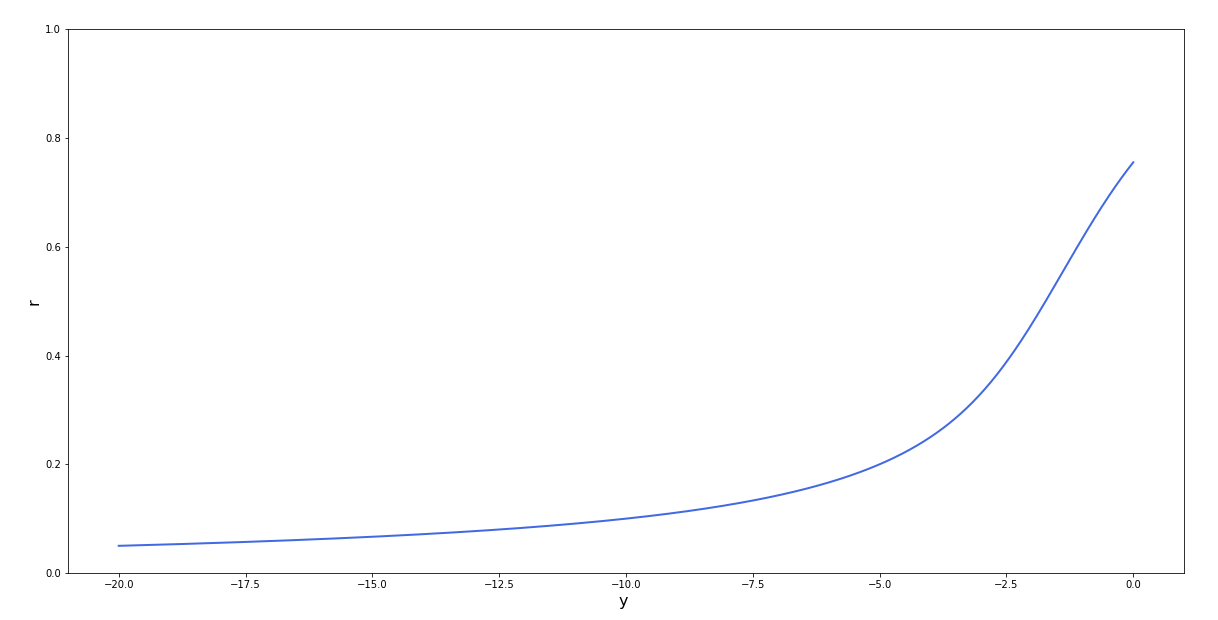
\includegraphics[width=1\textwidth]{tnorm_r}
	\caption{The relation between $r$ and $y$}
	\label{fig:tnorm_r}
\end{figure}
To find optimal revenue for truncated normal distribution, we consider an alternative way by using \textit{virtual valuation}. Previously we compute the optimal reserve price by maximize the expected revenue formula, because of the simplicity of uniform distribution, the equation of expected revenue is concave and simple to compute the derivative. However for truncated normal distribution, it is not easy to programme this way, therefore based on Myerson optimal auction the optimal reserve price is the price which makes the \textit{virtual valuation} equal 0. The \textit{virtual valuation} is defined as\\
\textbf{Definition 2.2} The \textit{virtual valuation} of bidder $i$ with valuation $v_i$ is 
\begin{center}
	$\psi_i(v_i) = v_i - \frac{1-F_i(v_i)}{f_i(v_i)}$ 
\end{center}
In our case, we only have one bidder, so just use $v$ instead of $v_i$, then we can write $\psi(v) = v - \frac{1-F_t (v)}{f_t (v)}$, and the optimal reserve price $p_{opt} = \psi^{-1}(0)$. During the experiments, we use numerical solver to solve this equation $\psi(v) = 0$ to get $p_{opt}$.\\

\subsection{Truncated Normal distribution is MHR}
One assumption of Myerson optimal auction is that the \textit{virtual valuation} needs to be regular, which means the \textit{virtual valuation} is non-decreasing in values. Thus we need to prove the regularity of the \textit{virtual valuation} for truncated normal distribution and to prove the regularity we can also prove that the truncated normal distribution is a MHR distribution, because MHR implies regularity. Below we show our proof for TN$(\hat{\mu}, \hat{\sigma}^2, 0, \infty)$ is MHR distribution,

\begin{proof}
Hazard rate for this truncated normal distribution is $h(v) = \frac{f_t(v)}{1 - F_t(v)}$, to prove it is non-decreasing, we can take its first derivative and see if the first derivative is nonnagative or not (here we assume $v \geqslant 0$):
\begin{equation}\notag
\begin{split}	
	h^{'}(v) &=\frac{f_t^{'}(v)}{1 - F_t(v)}  + \frac{f_t(v)\cdot F_t^{'} (v)}{(1 - F_t(v))^2}\\&= \frac{f_t^{'}(v)}{1 - F_t(v)}  + \frac{f_t^{2}(v)}{(1 - F_t(v))^2} \\&=\frac{ f_t^{'}(v)(1 - F_t(v)) + f_t^{2}(v)}{(1 - F_t(v))^2}
\end{split}
\end{equation} 
Clearly the denominator is nonnegative, so we only need to check the nominator, also $f_t(v) = \frac{1}{\hat{\sigma}} \frac{\phi(\frac{v-\hat{\mu}}{\hat{\sigma}})}{1 - \Phi(\frac{-\hat{\mu}}{\hat{\sigma}})}$ and $F_t(v) =  \frac{\Phi(\frac{v-\hat{\mu}}{\hat{\sigma}}) - \Phi(\frac{-\hat{\mu}}{\hat{\sigma}})}{1 - \Phi(\frac{-\hat{\mu}}{\hat{\sigma}})}  $,then:
\begin{equation}\notag
	\begin{split}	
		f_t^{'}(v)(1 - F_t(v)) + f_t^{2}(v)&=\frac{1}{\hat{\sigma}} \frac{-\frac{v-\hat{\mu}}{\hat{\sigma}^2}\phi(\frac{v-\hat{\mu}}{\hat{\sigma}})}{1 - \Phi(\frac{-\hat{\mu}}{\hat{\sigma}})} \cdot \frac{1 - \Phi(\frac{v-\hat{\mu}}{\hat{\sigma}})}{1 - \Phi(\frac{-\hat{\mu}}{\hat{\sigma}})} + \frac{\phi^2(\frac{v-\hat{\mu}}{\hat{\sigma}})}{\hat{\sigma}^2 (1 - \Phi(\frac{v-\hat{\mu}}{\hat{\sigma}}))^2} \\&= \frac{-\frac{v-\hat{\mu}}{\hat{\sigma}}\cdot \phi(\frac{v-\hat{\mu}}{\hat{\sigma}})\left(1 - \Phi(\frac{v-\hat{\mu}}{\hat{\sigma}})\right) + \phi^2(\frac{v-\hat{\mu}}{\hat{\sigma}})}{\hat{\sigma}^2 (1 - \Phi(\frac{-\hat{\mu}}{\hat{\sigma}}))^2}
	\end{split}
\end{equation} 
Now again we only need to prove the nominator is nonnegative or not. We consider it into two cases:

\begin{equation}\notag
	\begin{split}		
		-\frac{v-\hat{\mu}}{\hat{\sigma}}\cdot \phi(\frac{v-\hat{\mu}}{\hat{\sigma}})\left(1 - \Phi(\frac{v-\hat{\mu}}{\hat{\sigma}})\right) + \phi^2(\frac{v-\hat{\mu}}{\hat{\sigma}})
	\end{split}
\end{equation} 

\begin{itemize}
	\item Case 1: if $v \leqslant \hat{\mu}$, then $-\frac{v-\hat{\mu}}{\hat{\sigma}} \geqslant 0$,\\ we know $\phi(\frac{v-\hat{\mu}}{\hat{\sigma}}), 1-\Phi(\frac{v-\hat{\mu}}{\hat{\sigma}})$ is nonnegative, then $-\frac{v-\hat{\mu}}{\hat{\sigma}}\cdot \phi(\frac{v-\hat{\mu}}{\hat{\sigma}})(1 - \Phi(\frac{v-\hat{\mu}}{\hat{\sigma}})) + \phi^2(\frac{-\hat{\mu}}{\hat{\sigma}})$ is nonnegative
	\item Case 2: if  $v > \hat{\mu}$, then $\frac{v-\hat{\mu}}{\hat{\sigma}} > 0$ and set $x = \frac{v-\hat{\mu}}{\hat{\sigma}}$,\\
	 we know that Q-funtion is defined as $Q(x) = 1- \Phi(x)$, and it is bounded when $x > 0$,\begin{center}
	 	$\left( \frac{x}{1+x^2} \right)\phi(x) < Q(x) <\frac{\phi(x)}{x}$
	 \end{center}  thus \\ $-\frac{v-\hat{\mu}}{\sigma}\cdot \phi(\frac{v-\hat{\mu}}{\hat{\sigma}})(1 - \Phi(\frac{v-\hat{\mu}}{\hat{\sigma}})) + \phi^2(\frac{v-\hat{\mu}}{\hat{\sigma}})$ \vspace{2mm} \\$= -x\phi(x)(1-\Phi(x)) + \phi^2(x)$\vspace{2mm}\\$=-x\phi(x)Q(x) + \phi^2(x) > -x\phi(x)\cdot \frac{\phi(x)}{x} + \phi^2(x)  = -\phi^2(x) + \phi^2(x) = 0$\\ the expression is nonnegative.
\end{itemize}
 In both case, we prove that the nominator is nonnegative, thus the first derivative of truncated normal hazard rate is nonnegative, which means its hazard rate is monotone non-decreasing, and truncated normal distribution is a MHR distribution. Regularity assumption satisfied.
\end{proof}
\subsection{Result of experiment: TBC}
We experiment different truncated normal distributions with different $r$ values, and evaluate the corresponding DAPXs. In the implementation, we need to assign values to $\hat{\mu}, \hat{\sigma}$, in order to have different distributions, first we can set either of them to a fix value, in our case, we set $\hat{\mu}$ fixed and gradually increase $\hat{\sigma}$. As we derive in previous section, $r$ is a function of $\frac{\hat{\sigma}}{\hat{\mu}}$, only related to the ratio of $\hat{\mu}$ and $\hat{\sigma}$, so without loss we can set $\hat{\mu} = 1$. We plot the DAPX of truncated normal distributions and the theoretical $\rho_D$ in two plots: the left plot with small values of $r$ and the right with lager values of $r$. \cref{fig:tnorm_dapx_r} shows how these two values increase with $r$ increases. $\rho_D$ increases really fast while the experimental DAPX remains small. Since we gradually increase $\hat{\sigma}$, we can see the increment in \cref{fig:tnorm_dapx_r} is not uniform. Thus we also plot the results with parameter $\hat{\sigma}$. The left figure in \cref{fig:tnorm_dapx_s} shows the results with small $\hat{\sigma}$, while the right one is with larger $\hat{\sigma}$. Previously we find out $r$ is upper bounded, therefore $\rho_D$ is also upper bounded, and we can observe a clear convergence in \cref{fig:tnorm_dapx_r} and \cref{fig:tnorm_dapx_s}. We can also notice that the DAPX of truncated normal is also bounded. Our experiment shows the upper bound of DAPX of truncated normal is approximate 1.1522 for $r = 0.7555$.

\begin{figure}[H]
	\centering
	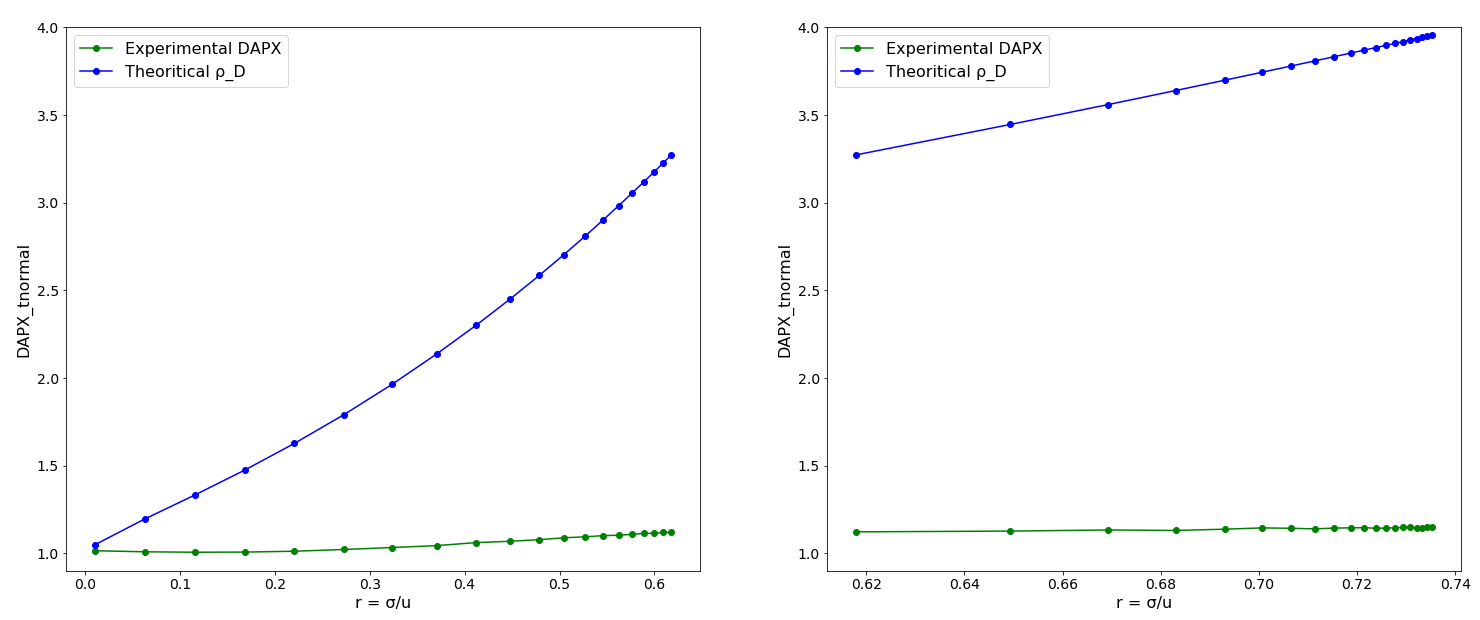
\includegraphics[width=1\textwidth]{tnorm_dapx_r}
	\caption{DAPX of truncated normal distribution versus $\rho_{D}$ with different $r$ values}
	\label{fig:tnorm_dapx_r}
\end{figure}
\begin{figure}[H]
	\centering
	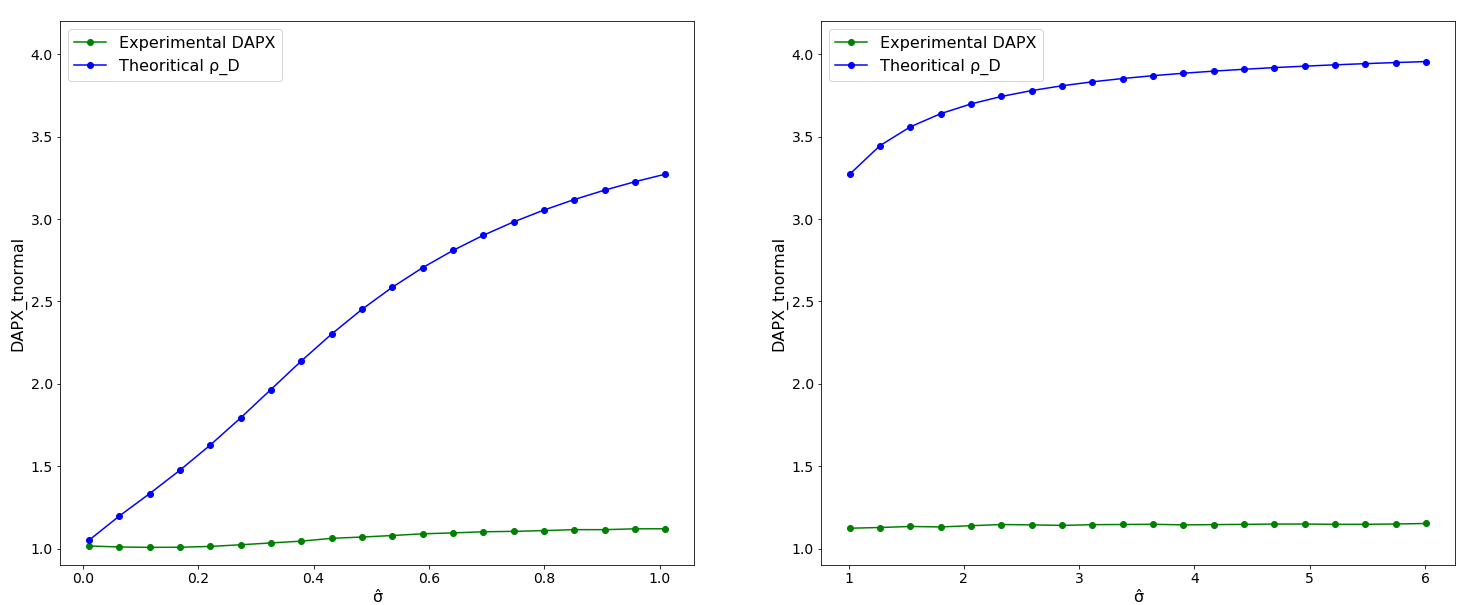
\includegraphics[width=1\textwidth]{tnorm_dapx_s}
	\caption{DAPX of truncated normal distribution versus $\rho_{D}$ with different $\hat{\sigma}$ values}
	\label{fig:tnorm_dapx_s}
\end{figure}

\section{Pareto distribution}
Here we also want to consider Pareto distribution. This distribution can possible be used in description of auction data when most bids are consetrated at lower values while high bid is hardly to occur. \\
Pareto distribution is defined by two parameters $x_m>0, c>0$ and $x \in [x_m, \infty]$. To simplify, we choose the scale parameter $x_m = 1$ and denote this Pareto distribution as Pareto(1) due to its support range. Next we can write corresponding PDF and CDF as following
\begin{equation}\notag
f(x) = \frac{c}{x^{c+1}} 
\end{equation} 
and 
\begin{equation}\notag
F(x) = 1- \frac{1}{x^c}
\end{equation} 
Another special property of Pareto distribution is that when parameter $c \leqslant 1$, it does not have a mean (the mean is infinite), in addition, when $c \leqslant 2$ its variance is infinite too. Thus in order to have a valid $r$, we assume the parameter $c > 2$. Then the mean and standard deviation of this Pareto distribution are
\begin{center}
	$\mu = \frac{c}{c-1} $ \hspace{2cm} $\sigma = \sqrt{\frac{c}{(c-1)^2(c-2))}}$
\end{center}
We first determine the optimal reserve price for this Pareto distribution. We use Myersons optimal operator again
\begin{equation}\notag
\text{OPT}\left(F\right) = \sup_{p \geqslant 1} \text{REV}(p;F) = \sup_{p \geqslant 1} p \cdot \left(1-\left(1- \frac{1}{p^c}\right)\right) =\sup_{p \geqslant 1} \ \frac{1}{p^{c-1}}
\end{equation}
since $c>2$, then $\frac{1}{p^{c-1}}$ is monotone decreasing. When reserve price $p = 1$, we can achieve the maximum expected revenue, thus OPT$(F)$ = 1. Now let's check whether $r$ is bounded or not
\begin{equation}\notag
r = \frac{\sigma}{\mu} = \frac{\sqrt{\frac{c}{(c-1)^2(c-2))}}}{\frac{c}{c-1} } = \frac{1}{\sqrt{c(c-2)}}
\end{equation}
As we can see from the expression, when $c \to 2$, $r \to \infty$, thus r is unbounded and our theoretical bound $\rho_D$ is also unbounded. However our experiment shows the DAPX of the Pareto distribution is not unbounded, as we can see figure....., so we write down the expression for DAPX explicitly:
\begin{equation}\notag
\begin{split}
	\text{DAPX} &= \frac{\text{OPT}(F)}{\text{REV}(F)} =\frac{1}{p_D(1-F(p_D))} =\frac{1}{p_D\left(1-\left(1-\frac{1}{p_D^c}\right)\right)}\\& = p_D^{c-1}	 = (\mu \frac{\rho_{D}}{2\rho_{D}  -1})^{c-1} = \left(\frac{c}{c-1} \cdot \frac{1}{2 - \frac{1}{\rho_{D}}}\right)^{c-1}\\& = \left( (1 + \frac{1}{c-1}) \cdot\frac{1}{2 - \frac{1}{\rho_{D}}}\right)^{c-1}
\end{split}
\end{equation} 
From the expression, when $c \to 2$, we know $r \to \infty$ and $\rho_D  \to \infty$ also, then DAPX $\to 1$; when $c \to \infty$, and $r \to 0$ and $\rho_D  \to 1$, so DAPX $\to 1$ also. This matches the results in both \cref{fig:pareto_dapx2} and \cref{fig:pareto_dapx3}. \cref{fig:pareto_dapx1} shows the experimental DAPX comparing to $\rho_D$, as we can see, the DAPX of Pareto(1) remains small while $\rho_D$ increases exponentially. \cref{fig:pareto_dapx2} shows the experimental DAPX by itself, as we can see, the DAPX remains around 1 and we observe a clear upper bound. To see more details how DAPX values under small $r$ values, we run the experiment with 50 steps at range (0, 2) of $r$. Results are represented in \cref{fig:pareto_dapx3}, and from the experiment the upper bound of Pareto(1) DAPX $\approx 1.1416$ to 4 decimals for $r = 0.2700$.     
\begin{figure}[H]
	\centering
	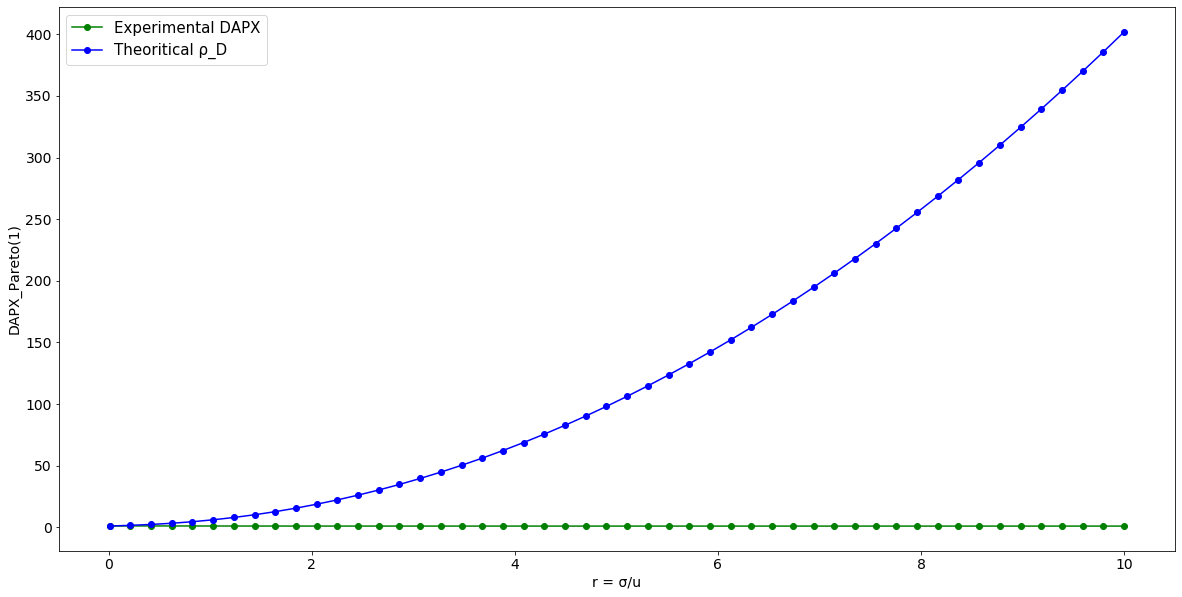
\includegraphics[width=1\textwidth]{pareto_dapx1}
	\caption{DAPX of Pareto(1) distribution versus $\rho_D$}
	\label{fig:pareto_dapx1}
\end{figure}
\begin{figure}[H]
	\centering
	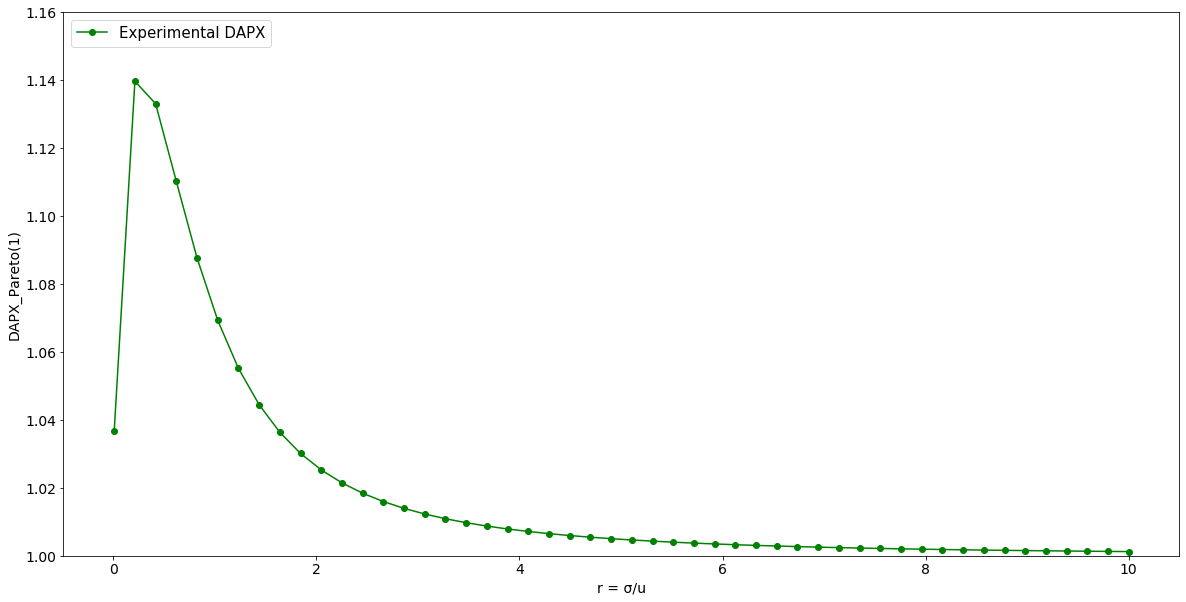
\includegraphics[width=1\textwidth]{pareto_dapx2}
	\caption{DAPX of Pareto(1) distribution with $r$}
	\label{fig:pareto_dapx2}
\end{figure}
\begin{figure}[H]
	\centering
	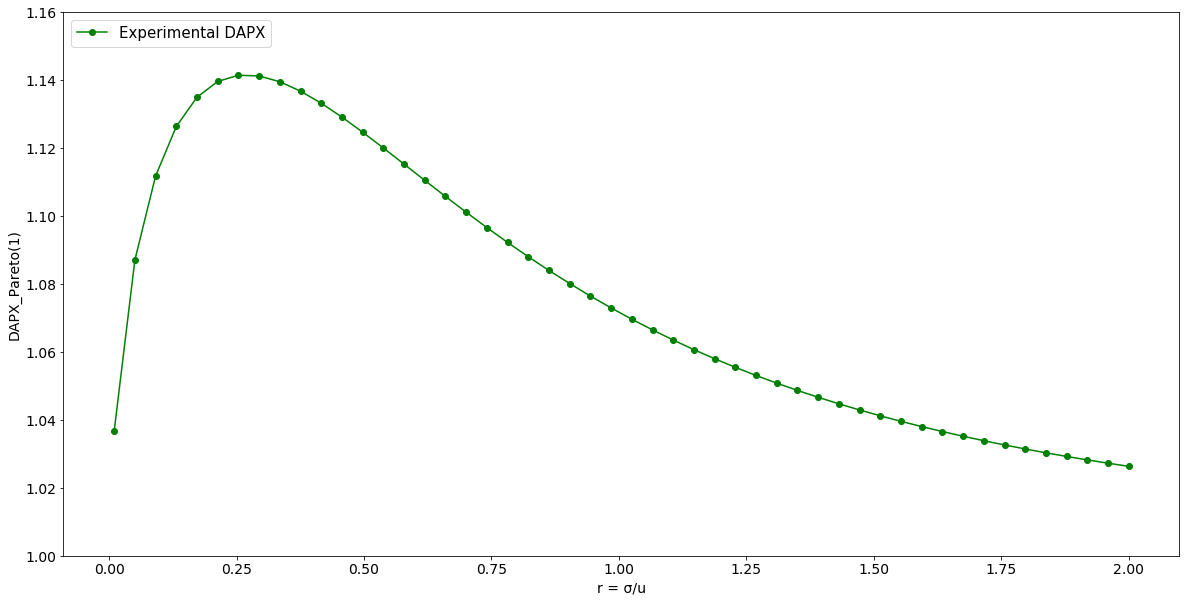
\includegraphics[width=1\textwidth]{pareto_dapx3}
	\caption{DAPX of Pareto(1) distribution when $r$ remains small}
	\label{fig:pareto_dapx3}
\end{figure}



\subsection{Pareto Extension}
We usually consider all the valuation is non-negative, therefore we would like to modify the previous Pareto distribution to have support [0,  $\infty$), which means shifting the distribution  to the left by 1. Let's denote this distribution as Pareto(0) and its PDF and CDF are
\begin{equation}\notag
f(x) = \frac{c}{(x+1)^{c+1}} 
\end{equation} 
and 
\begin{equation}\notag
F(x) = 1- \frac{1}{(x+1)^c}
\end{equation} 
Below we make sure it is a valid distribution:
\begin{align}\notag
	\int_{0}^{\infty} f(x) dx &= 1- \frac{1}{(x+1)^c} \Biggr|_{0}^{\infty}  = 1 - 0 -(1-\frac{1}{1}) = 1 \\ \notag  F(0) &= 1- \frac{1}{(0+1)^c} =0 \\ \notag  \lim_{x \to \infty} F(x) &= \lim_{x \to \infty} 1- \frac{1}{(x+1)^c} = 1
\end{align}
We can derive  mean and standard deviation of Pareto(0) from Pareto(1). We denote $E[X], Var[X]$ are mean and variance of Pareto(1) , then $E[X-1], Var[X-1]$ is the mean and variance for Pareto(0). We get $E[X-1] = E[X] - 1$ and $Var[X-1] = Var[X]$, thus from this relation, we can write down the formula for $\mu, \sigma$
\begin{center}
	$\mu = \frac{1}{c-1}$ \hspace{1cm} and \hspace{1cm}$\sigma = \sqrt{\frac{c}{(c-1)^2(c-2)}}$
\end{center}
This time $p_{opt} =\displaystyle\ \arg \max_{\substack{p \geqslant 0}} \  p(1 - (1-\frac{1}{(p+1)^c})) =\displaystyle\arg \max_{\substack{p \geqslant 0}} \  \frac{p}{(p+1)^c}$, to find $p_{opt}$, we take the first derivative of $\frac{p}{(p+1)^c}$, and check if the maximum exists or not.
\begin{equation}\notag
	\frac{p}{(p+1)^c}' = \frac{1}{(p+1)^c} - \frac{pc}{(p+1)^{c+1}} = \frac{1 - p(c-1)}{(p+1)^{c+1}}
\end{equation} 
Since $p \geqslant 0, c>2$, when $p < \frac{1}{c-1}$, then $\frac{p}{(p+1)^c}' > 0$, which means $\frac{p}{(p+1)^c}$ monotonously increases at [0,$\frac{1}{c-1}$), while $p > \frac{1}{c-1}$, then $\frac{p}{(p+1)^c}' < 0$ means $\frac{p}{(p+1)^c}$ monotonously decreases at ($\frac{1}{c-1}$,$\infty$). Therefore the maximum value can be achieved when $p = \frac{1}{c-1}$.
Then $p_{opt} = \frac{1}{c-1}$, we can also write down the optimal revenue:
\begin{equation}\notag
	\text{OPT} (F)=  \frac{1}{c-1} \cdot \frac{1}{(\frac{1}{c-1}+1)^c} = \frac{(c-1)^{c-1}}{c^c}
\end{equation}
and $r$ 
\begin{equation}\notag
r = \frac{\sigma}{\mu} = \frac{\sqrt{\frac{c}{(c-1)^2(c-2)}}}{\frac{1}{c-1} } = \sqrt{\frac{c}{c-2}} =\sqrt{\frac{1}{1-\frac{2}{c}}} 
\end{equation}
We can get similar conclusion as before: if $c \to 2$, $r \to \infty$; if $c \to \infty$, $r \to 1$. Therefore $r$ is also unbounded in this case. Then we write down DAPX for Pareto(0) explicitly
\begin{equation}\notag
	\begin{split}
		\text{DAPX} &= \frac{\text{OPT}(F)}{\text{REV}(F)} =\frac{\frac{(c-1)^{c-1}}{c^c}}{p_D(1-F(p_D))}\\ \\ &= \frac{(c-1)^{c-1}}{c^c} \cdot \frac{(p_D +1)^c}{p_D}
	\end{split}
\end{equation} 
where $p_D = \frac{1}{c-1} \cdot \frac{\rho_{D} }{2\rho_{D} -1}$, from above expression, it is hard to see if an upper bound for DAPX of Pareto(0) exists or not. If we plot above expression, from \cref{fig:pareto_dapx_r}, we can see DAPX is a function of $r$ which is monotone decreasing, so it is bounded when $r \to 1$. We can find this upper bound using the experiment by setting parameter $c$ to a very large number, so $r \to 1$, and our result shows the Pareto(0) DAPX is 1.1638 to 4 decimal places for $c = 10^ {10}$.
\begin{figure}[H]
	\centering
	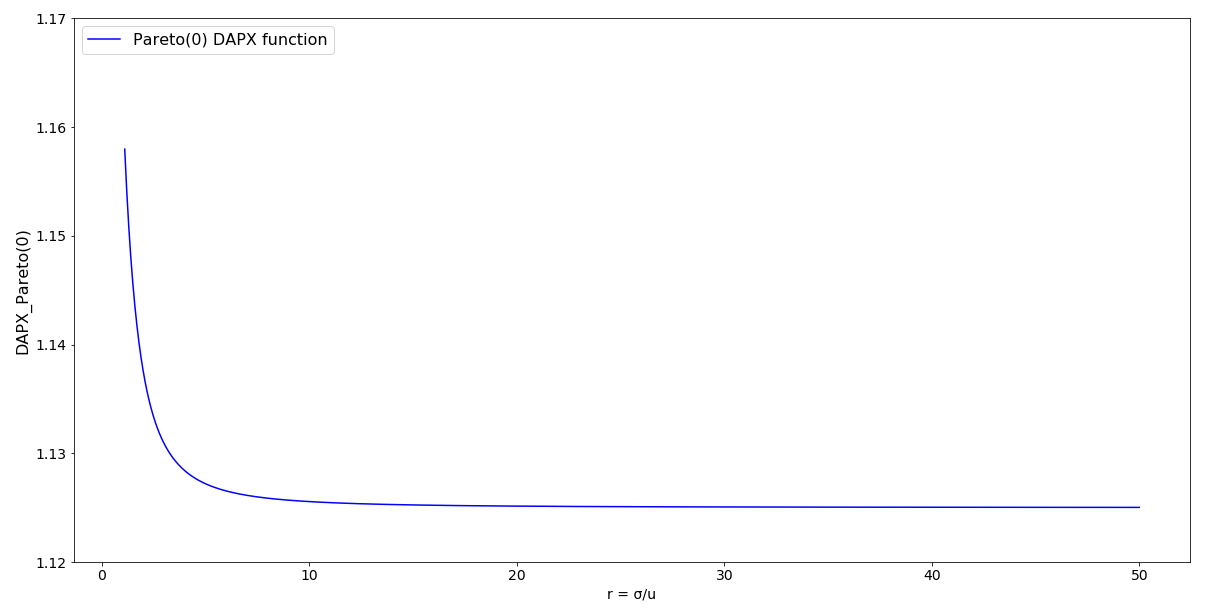
\includegraphics[width=1\textwidth]{pareto_dapx_r}
	\caption{Pareto(0) DAPX function}
	\label{fig:pareto_dapx_r}
\end{figure}
\subsection{Result}
First we show the results of the experimental DAPX and $\rho_D$ with $r \in (0,10)$. From \cref{fig:pareto_dapx_r_large}, as we can see $\rho_D$ increase exponentially with $r$, while the experimental DAPX remain small(around 1). In the second \cref{fig:pareto_dapx_r_small}, we can see more details of these two values when $r \to 1$. 
\begin{figure}[H]
	\centering
	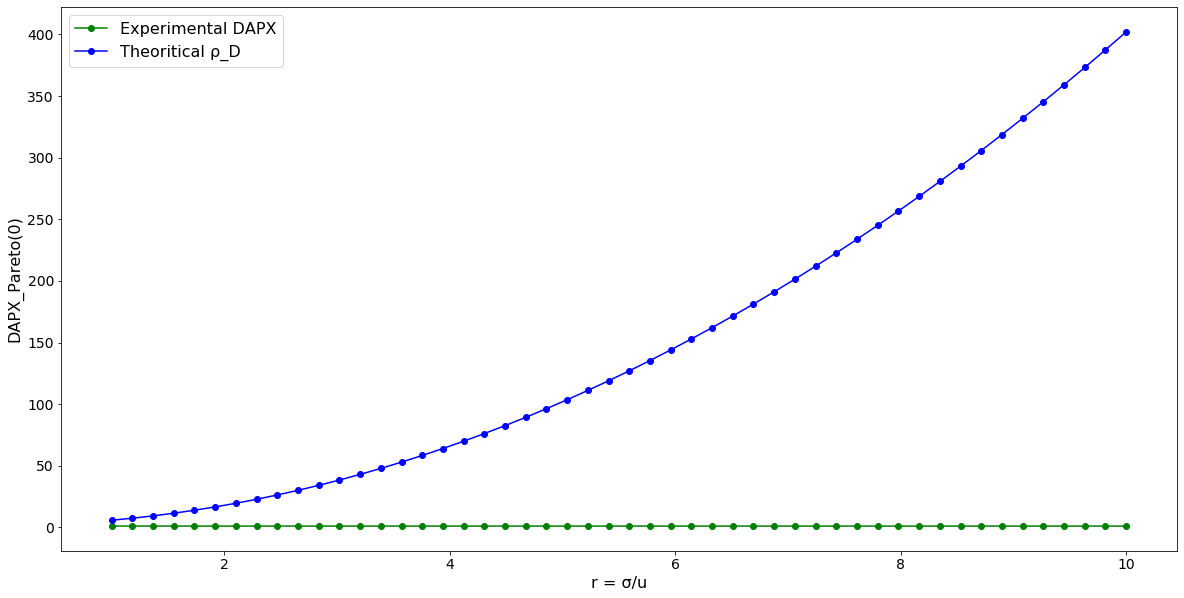
\includegraphics[width=1\textwidth]{pareto_dapx_r_large}
	\caption{Pareto(0) DAPX when $r \in (0,10)$}
	\label{fig:pareto_dapx_r_large}
\end{figure}
\begin{figure}[H]
	\centering
	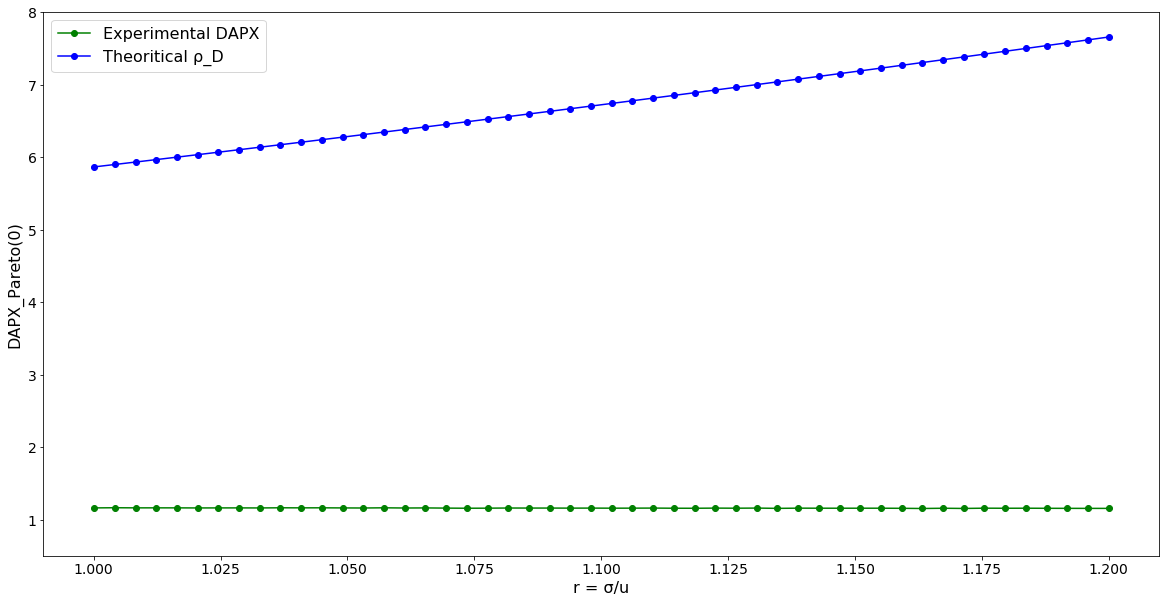
\includegraphics[width=1\textwidth]{pareto_dapx_r_small}
	\caption{Pareto(0) DAPX when $r \in (1, 1.2)$}
	\label{fig:pareto_dapx_r_small}
\end{figure}


\section{Summary of Deterministic SBSI Auction}
From above evaluation on different distributions, we notice that for most of these distributions, $r$ is upper bounded, which also means, our theoretical $\rho_D$ and our experimental DAPX have also an upper bound. \cref{tab:dapxbound} represent our foundlings from our evaluation(keep 4 decimals): 

\begin{center}
	\begin{table}[hbt]
		\begin{tabular}{ | m{3.2cm} | m{2.8cm}| m{3cm} |m{4cm}|  } 
		\hline
		\textbf{Distribution}	&	\textbf{r upper bound}  & \textbf{Theoritical $\rho_D$ upper bound} & 	\textbf{Experimental DAPX upper bound}  \\ 
		\hline
		Uniform distribution&$\frac{1}{\sqrt{3}}$& 3.0593 & 1.1919 \\ 
		\hline
		Truncated normal distribution & $\frac{ \sqrt{1-4\phi(0)^2}}{2\phi(0)}$ & 4.0836& 1.1511 \\ 
		\hline
		 Pareto distribution ($x \in \left[1,\infty \right)$)& $\infty$ & $\infty$& 1.1416 \\
		\hline
		 Pareto distribution ($x \in \left[0,\infty \right)$)& $\infty$ & $\infty$& 1.1638 \\
		\hline
		\end{tabular}
		\caption{Upper bound table}
		\label{tab:dapxbound}
	\end{table}
\end{center}
We discuss the Uniform distribution DAPX in . There are two cases, since the upper bound of $r$ is $\frac{1}{\sqrt{3}}$ when $\frac{b}{a} \rightarrow \infty$, therefore in this case, $\frac{b}{2} \geqslant a$, then DAPX =  $\frac{ ( \sqrt{3}r +1)^{2}}{4 \cdot \frac{ \rho_{D}}{2\rho_{D}-1}\cdot( \sqrt{3}r+ 1-\frac{\rho_{D}}{2\rho_{D}-1})}$. We subsititute $r = \frac{1}{\sqrt{3}}$ and $\rho_D = 3.5936$ into this equation, The upper bound for DAPX of uniform distribution is 1.1931. Our experimental number in \cref{tab:dapxbound} matches this number. We can also explicitly compute the DAPX upper bound for Truncated normal distribution using following equation:
\begin{equation}\notag
\text{DAPX} = \frac{\text{OPT}(F)}{\text{REV}(F)} =\frac{p_{opt}(1-F_t(p_{opt}))} {p_D(1-F_t(p_{D}))} 	
\end{equation} 
where $p_{opt}$ and $p_D$ can be determined explicitly with $r = 0.7555$. Then $\sup \text{DAPX} = 1.1515$, our experimental value matches this number. 


%%% Local Variables: 
%%% mode: latex
%%% TeX-master: "thesis"
%%% End: 